%%%%%%%%%%%%%%%%%%%%%%%%%%%%%%%%%%%%%%%%%%%%%%%%%
% ce-testsuite.tex
% 
% Latex source to be converted to HTML by tex4ht
%
%%%%%%%%%%%%%%%%%%%%%%%%%%%%%%%%%%%%%%%%%%%%%%%%%
\documentclass{article}

%%%%%%%%%%%%%%%%%%%%%%%%%%%%%%%%%%%%%%%%%%%%%%%%%
% PREAMBLE
%%%%%%%%%%%%%%%%%%%%%%%%%%%%%%%%%%%%%%%%%%%%%%%%%
% Import common configurations and custom functions
%%%%%%%%%%%%%%%%%%%%%%%%%%%%%%%%%%%%%%%%%%%%%%%%%
% PREAMBLE
%%%%%%%%%%%%%%%%%%%%%%%%%%%%%%%%%%%%%%%%%%%%%%%%%
\usepackage{hyperref}
\usepackage{listings}
\usepackage{color}
\usepackage[dvipsnames]{xcolor}
\usepackage{float}
\usepackage{graphicx}
\usepackage{tikz,tikz-dependency}
\usepackage{ifthen}
\usetikzlibrary{calc}
\usetikzlibrary{automata,positioning,external,shapes,arrows,chains,matrix,scopes,backgrounds}
\usepackage{enumerate}
% The following is for tikz externalization configuration which allows
% tikZ diagrams to render correctly while being processed by htlatex 
% http://tex.stackexchange.com/questions/158551/using-htlatex-with-tikz-dependency#158921
%%%%%%%%%%%%%%%%%%%%%%%%%%%%%%%%%%%%%%%%%%%%%%%%%
\tikzset{
    tex4ht inc/.style={
        /pgf/images/include external/.code={%
            \includegraphics[]{##1.svg}%
        }

    }
}
\tikzset{
 external/system call/.add={}
      ; inkscape -z -f "\image.pdf" -l "\image.svg"
}
\makeatletter
\@ifpackageloaded{tex4ht}{
    \tikzexternalize[mode=only graphics]
}{
    \tikzexternalize
}
\makeatother

% Removes section numbers
\makeatletter
\renewcommand\thesection{}
%\renewcommand\thesubsection{\@arabic\c@section.\@arabic\c@subsection}
\renewcommand\thesubsection{}
\makeatother

%%%%%%%%%%%%%%%%%%%%%%%%%%%%%%%%%%%%%%%%%%%%%%%%%
% COLOR DEFINITIONS
%%%%%%%%%%%%%%%%%%%%%%%%%%%%%%%%%%%%%%%%%%%%%%%%%
\tikzstyle{red}     = [fill=red!30!white]
\tikzstyle{orange}  = [fill=orange!30!white]
\tikzstyle{yellow}  = [fill=yellow!30!white]
\tikzstyle{green}   = [fill=green!30!white]
\tikzstyle{blue}    = [fill=blue!30!white]
\tikzstyle{teal}    = [fill=teal!30!white]
\tikzstyle{purple}  = [fill=purple!30!white]
\tikzstyle{magenta} = [fill=magenta!30!white]
\tikzstyle{gray}    = [fill=gray!30!white]
%\tikzstyle{black}   = [fill=black!30!white]

%%%%%%%%%%%%%%%%%%%%%%%%%%%%%%%%%%%%%%%%%%%%%%%%%
% DEFINE STACK COLORS
%%%%%%%%%%%%%%%%%%%%%%%%%%%%%%%%%%%%%%%%%%%%%%%%%
\definecolor{DEFINE_USR_COLOR}{HTML}{006699}
\definecolor{DEFINE_KRN_COLOR}{HTML}{003366}
\definecolor{DEFINE_HW_COLOR}{HTML}{000033}
\definecolor{DEFINE_CET_COLOR}{HTML}{339999}
\definecolor{DEFINE_CE_ARQ_COLOR}{HTML}{003333}

\tikzstyle{DK_COLOR}  = [fill=blue!30!white]
\tikzstyle{ARQ_COLOR} = [fill=gray!30!white]
\tikzstyle{OS_COLOR}  = [fill=black!50!white]
\tikzstyle{USR_COLOR} = [fill=DEFINE_USR_COLOR]
\tikzstyle{KRN_COLOR} = [fill=DEFINE_KRN_COLOR]
\tikzstyle{HW_COLOR}  = [fill=DEFINE_HW_COLOR]
\tikzstyle{CET_COLOR} = [fill=DEFINE_CET_COLOR]
\tikzstyle{CE_ARQ_COLOR} = [fill=DEFINE_CE_ARQ_COLOR]
\tikzstyle{HM_COLOR}  = [fill=cyan!30!white]
%%%%%%%%%%%%%%%%%%%%%%%%%%%%%%%%%%%%%%%%%%%%%%%%%
% STACK DIAGRAM DEFINITIONS
%%%%%%%%%%%%%%%%%%%%%%%%%%%%%%%%%%%%%%%%%%%%%%%%%
\tikzstyle{layer}      = [rectangle, thick, rounded corners]
\tikzstyle{core_stack} = [layer, minimum width=11cm,minimum height=1cm, text = white]
\tikzstyle{user_stack} = [layer, minimum width=4cm,minimum height=1cm]
\tikzstyle{app_stack}  = [layer, minimum width=4.5cm,minimum height=3cm]
\tikzstyle{container}  = [layer, purple,minimum width=0.5cm,minimum height=0.5cm]

\tikzstyle{OS_LAYER}  = [app_stack]
\tikzstyle{ARQ_LAYER} = [app_stacK]
\tikzstyle{CET_LAYER} = [user_stack, CET_COLOR]
\tikzstyle{USR_LAYER} = [core_stack, USR_COLOR, minimum height=4.5cm, label={[label distance=-0.75cm]270:\color{white}Userspace}]
\tikzstyle{KRN_LAYER} = [core_stack, KRN_COLOR, below= 0cm of USR]
\tikzstyle{HW_LAYER}  = [core_stack, HW_COLOR, below of=KRN]
\tikzstyle{DK_LAYER}  = [user_stack, DK_COLOR]
\tikzstyle{HM_LAYER}  = [user_stack, HM_COLOR]

%%% NEW DEFS
\tikzstyle{OS_LAYER2} = [app_stack, OS_COLOR,fill=black!50!white, label={[label distance=-0.75cm]270:OpenShift}]

\tikzstyle{c_temp} = [layer,minimum width=0.5cm,minimum height=0.5cm]
\tikzstyle{c_empt} = [c_temp]
\tikzstyle{c_move} = [c_temp, draw, dotted]
\tikzstyle{c_full} = [c_temp, purple, draw=black, thin]
\tikzstyle{mw}     = [minimum width=5.0cm]

\tikzstyle{c}    = [container, draw=black, thin]
\tikzstyle{pod}  = [thick, opacity=0.5, rounded corners]
\tikzstyle{NS}   = [thick, draw, dotted] %Namespace
\tikzstyle{blank}= [c_temp, OS_COLOR, thick, c_move]
\tikzstyle{pod}  = [thick, opacity=0.4, rounded corners, circle]
\tikzstyle{box} = [rectangle, thick, rounded corners, text= white]
\tikzstyle{link} = [-, thick, opacity=0.3]

\definecolor{keyword}{rgb}{0,0,0}
\definecolor{comment}{rgb}{0,0,0}
\definecolor{string}{rgb}{0,0,0}

% lstlisting configs for code syntax formatting
\lstdefinestyle{Java} {
  frame=tb,
  language=Java,
  aboveskip=3mm,
  belowskip=3mm,
  showstringspaces=false,
  columns=flexible,
  basicstyle={\large\ttfamily},
  numbers=none,
  numberstyle=\textcolor{gray},
  keywordstyle=\textcolor{red!75},
  commentstyle=\textcolor{dkgreen},
  stringstyle=\textcolor{blue},
  moredelim=[is][\textcolor{black!75}]{|}{|},
  breaklines=false,
  breakatwhitespace=true,
  tabsize=3,
  belowskip=-0.5em %\baselineskip
}

\lstdefinestyle{shell} {
  basicstyle=\ttfamily,
  showstringspaces=false,
  keywordstyle=\textcolor{keyword},
  commentstyle=\textcolor{comment},
  stringstyle=\textcolor{string},
  belowskip=-\baselineskip
  %belowskip=-\baselineskip
}

%%%%%%%%%%%%%%%%%%%%%%%%%%%%%%%%%%%%%%%%%%%%%%%%
% Tikz Functions
%%%%%%%%%%%%%%%%%%%%%%%%%%%%%%%%%%%%%%%%%%%%%%%%
\newcommand{\containers}[4] {
  \xdef\cmax{7}
  \def\id{#1}                   % #1 = id 
  \pgfmathsetmacro\nc{int(#2)}  % #2 = number of containers
  \pgfmathsetmacro\nfc{int(#3)} % #3 = number of full containers 
  \tikzstyle{LOCATION} = {#4}   % #4 = location
  \node[#4] (loc) {}; 

  \node[LOCATION] (loc) {};
  % Initialize container nodes
  \foreach \x in {0,...,7}{
    \node[] (C\x_\id) {};
  }

  \xdef\sp{loc};     % starting position
  \xdef\ct{c_full}; % container type
  \foreach \x in {0,...,\cmax} {
    {\ifthenelse{\x < \nc}
      { {\ifthenelse{\x < \nfc }
          {\xdef\ct{c_full};}
          {\xdef\ct{c_move};}
        }
      }
      { \xdef\ct{c_empt};}
    }
    \node[\ct, right=of \sp] (C\x_\id) {};
    \xdef\sp{C\x_\id};
  };

  %{\ifthenelse{\nc < 4}{}{
  %Container label with spanning arrows
  \node[fit=(C0_\id)(C1_\id)(C2_\id)(C3_\id)(C4_\id)(C5_\id)(C5_\id)(C6_\id)(C7_\id)] (all) {};
  \node[above= -0.15cm of all.north ] (C_LABEL_\id) {\small Containers};
  \path[->, to path={-| (\tikztotarget)}]
  (C_LABEL_\id.west) edge (C0_\id.north)
  (C_LABEL_\id.east) edge (C7_\id.north);
  
}

\newcommand{\moby}[4] {
  \xdef\cmax{7}
  \def\id{#1}                   % #1 = id 
  \pgfmathsetmacro\nc{int(#2)}  % #2 = number of containers
  \pgfmathsetmacro\nfc{int(#3)} % #3 = number of full containers 
                                % #4 = location
  % Initialize container nodes
  \foreach \x in {0,...,7}{
    \node[] (C\x_\id) {};
  }
  % Instantiate moby and container nodes
  \node[DK_LAYER, DK_COLOR, #4] (DK_\id) {Moby};
  \node[above left= 0.1cm and 0cm of DK_\id.north west] (sp) {};

  \xdef\sp{sp};     % starting position
  \xdef\ct{c_full}; % container type
  \foreach \x in {0,...,\cmax} {
    {\ifthenelse{\x < \nc}
      { {\ifthenelse{\x < \nfc }
          {\xdef\ct{c_full};}
          {\xdef\ct{c_move};}
        }
      }
      { \xdef\ct{c_empt};}
    }
    \node[\ct, right=of \sp] (C\x_\id) {};
    \xdef\sp{C\x_\id};
  };

  {\ifthenelse{\nc < 4}{}{
  %Container label with spanning arrows 
  \node[above= 0.5cm of DK_\id.north ] (C_LABEL_\id) {Containers};
  \path[->, to path={-| (\tikztotarget)}]
  (C_LABEL_\id.west) edge (C0_\id.north)
  (C_LABEL_\id.east) edge (C7_\id.north);
  }};
}
\newcommand{\host}[4]{
  \def\id{#1}  % #1 = id
  \def\nc{#2}  % #2 = number of containers
  \def\nfc{#3} % #3 = number of full containers
               % #4 = location
  % Initialize nodes
  \foreach \x in {0,...,7}
    \node[] (C\x_\id) {};
    \node[] (DK_\id) {};
    \node[] (OS_\id) {};

  \node[OS_LAYER,fit=(DK_\id)] at (#4) (OS_\id) {};
  \moby{#1}{#2}{#3}{above = 0cm of OS_\id.center, anchor=center};
  \node[HM_LAYER, mw, below= 0cm of OS_\id.south, anchor=north] (HM_\id) {Host Machine \id};
}

\newcommand{\OpenShift}[4]{
  \def\id{#1}  % #1 = id
  \def\nc{#2}  % #2 = number of containers
  \def\nfc{#3} % #3 = number of full containers
               % #4 = location
  % Initialize nodes
  \foreach \x in {0,...,7}
    \node[] (C\x_\id) {};
    \node[] (DK_\id) {};
    \node[] (OS_\id) {};

  \node[OS_LAYER,fit=(DK_\id), #4] (OS_\id) {};
  \moby{#1}{#2}{#3}{above = 0cm of OS_\id.center, anchor=center};
}

\newcommand{\Arquillian}[2]{
  \def\id{#1}  % #1 = id
               % #2 = location

  \node[] (CET_\id) {};
  \node[ARQ_LAYER, fit=(CET_\id), #2] (ARQ_\id) {};
  \node[CET_LAYER, above = 0cm of ARQ_\id.center, anchor=center] (CET_\id) {CE-Testsuite};
}

\newcommand{\pods}[5]{
  \xdef\id{#1}
  \pgfmathtruncatemacro{\numPods}{#2-1}
  \xdef\numCons{#3-1};
  \pgfmathtruncatemacro{\cpp}{2 - 1} %containers per pod
  \xdef\cfit{} % containers for pod to fit
  \xdef\pfit{} % pods for namespace to fit

  \node[#4] (BASE) {};
  \xdef\lcp{BASE}; % last container position
  \xdef\sbc{}; % space between container
  \pgfmathsetmacro\r{#3}
 % Initialize pods
  \foreach \x in {0,...,\numPods}{
    \pgfmathsetmacro\pods{int(#2 - \x)}
    {\ifthenelse{\r > \pods }
    { % if 
      \xdef\numCons{1}
      \pgfmathsetmacro\r{int(\r - 2)}
      \xdef\r{\r}
    }
    { % else
      \xdef\numCons{0};
      \pgfmathsetmacro\r{int(\r - 1)}
      \xdef\r{\r}
    }
    };
    %\node[] at (-5,\x) {\r \pods \numCons};

    \foreach \y in {0,...,\numCons}{
      \node[c_full, right= \sbc of \lcp] (P\x_C\y_#1) {};
      \xdef\lcp{P\x_C\y_#1}
      \xdef\cfit{\cfit(P\x_C\y_#1)} % add container to be fitted
      \xdef\sbc{}; %space between containers
    }

    % randomly generate color for pod
    \pgfmathparse{rnd}
    \pgfmathtruncatemacro{\cc}{(\id)*0.4}
    \xdefinecolor{rColor}{rgb}{\cc, 0.7, \pgfmathresult}

    \node[pod, fill=rColor, fit=\cfit] (P\x_\id) {};
    %\pgfmathparse{rnd * \x}

    \xdef\cfit{};
    \xdef\sbc{0cm and 0.5cm}; %space between containers
    \xdef\pfit{\pfit(P\x_\id)} % add container to be fitted
    }
    #5
}

\newcommand{\namespace}[4]{
  \pods{#1}{#2}{#3}{#4}{\node[fit=\pfit] (NS_#1) {};};
  \node[NS, fit=\pfit] (NS_#1) {};
  \node[above=0cm of NS_#1.north] (NS_#1_LABEL) {Namespace #1};
  %\node[NS, fill=gray!10, fit=\pfit] (NS_#1) {};
  \pods{#1}{#2}{#3}{#4}{};
  %\pods{#1}{#2}{#3}{#4}{};
}

\newcommand{\cube}[4] {
  \def\id{#1}
  \def\size{#2}
  \def\color{#3}
  \tikzstyle{location} = [#4]

  \def\x{\size * 0.4}
  \def\y{\size * 0.5}
  \def\z{\size * 1.0}

  \tikzstyle{coor} = [shape=coordinate]
  \node[circle, location] (\id) {};

  \node[coor, below left =\x cm and \y cm of \id] (S_\id) {S};
  \node[coor, above=\z cm and 0cm of S_\id] (A_\id) {A};
  \node[coor, above right=\y cm and \x cm of A_\id] (B_\id) {B};
  \node[coor, above right=\y cm and \x cm of S_\id] (C_\id) {C};
  \node[coor, right=0.0cm and \z cm of S_\id] (D_\id) {D};
  \node[coor, above=\z cm and 0.0cm of D_\id] (E_\id) {E};
  \node[coor, above right=\y cm and \x cm of E_\id] (F_\id) {F};
  \node[coor, above right=\y cm and \x cm of D_\id] (G_\id) {G};

  \tikzstyle{face} = [black]

  \draw[face, fill=\color!30] (S_\id) -- (C_\id) -- (G_\id) -- (D_\id) -- cycle; % Bottom Face
  \draw[face, fill=\color!30] (S_\id) -- (A_\id) -- (E_\id) -- (D_\id) -- cycle; % Back Face
  \draw[face, fill=\color!10] (S_\id) -- (A_\id) -- (B_\id) -- (C_\id) -- cycle; % Left Face
  \draw[face, fill=\color!20,opacity=0.8] (D_\id) -- (E_\id) -- (F_\id) -- (G_\id) -- cycle; % Right Face
  \draw[face, fill=\color!20,opacity=0.6] (C_\id) -- (B_\id) -- (F_\id) -- (G_\id) -- cycle; % Front Face
  \draw[face, fill=\color!20,opacity=0.8] (A_\id) -- (B_\id) -- (F_\id) -- (E_\id) -- cycle; % Top Face

  \node[coor] (\id_center) at ($(S_\id)!0.5!(F_\id)$)  {};
  \node[coor] (\id_north)  at ($(A_\id)!0.5!(F_\id)$)  {};
  \node[coor] (\id_east)   at ($(D_\id)!0.5!(F_\id)$)  {};
  \node[coor] (\id_south)  at ($(S_\id)!0.5!(G_\id)$)  {};
  \node[coor] (\id_west)   at ($(S_\id)!0.5!(B_\id)$)  {};

  %\node[fit=(S_\id)(F_\id)] (\id) {};
  %\tikzstyle{cube}= [fit=(S_\id)(A_\id)(B_\id)(C_\id)(D_\id)(E_\id)(F_\id)(G_\id)];
  %\node[circle, draw, location] (test\id) {};
}

% Registry \regID is labeled in the format R<Registry number> 
% (e.g. R0 would represent Registry 0) while the cubes are 
% separated into labels of R\idC\row\col 
% (e.g. R0C00 Cube row 0 and col 0 of Registry 0)
\newcommand{\registry}[5] {
  \def\regID{#1}
  \pgfmathsetmacro{\cubesize}{#2};
  \pgfmathsetmacro{\rows}{int(#3 - 1)}
  \pgfmathsetmacro{\cols}{int(#4 - 1)}
  \tikzstyle{loc} = [#5]

  \node[loc] (LOCATION) {};

  \foreach \r in {0,...,\rows}{
    \foreach \c in {0,...,\cols}{
      \pgfmathsetmacro{\vdis}{\r * \cubesize}
      \pgfmathsetmacro{\hdis}{\c * \cubesize}
      %\pgfmathsetmacro{\num}{int(\c + (\r * #4))}
      %\node[above right= \vdis cm and \hdis cm of LOCATION] (Cuve\num R) {};
      \cube{\regID C\r \c}{\cubesize}{gray}{above right= \vdis cm and \hdis cm of LOCATION};
    }
  }

  \node[fit=(S_\regID C00) (F_\regID C\rows \cols)] (\regID) {};
  \node[above= -0.10cm of \regID] (\regID_label) {\small Registry};
}

%\newcommand{\template}[4] {
%  \def\tempID{#1}
%  \pgfmathsetmacro{\size}{#2}
%  \pgfmathsetmacro{\minWidth}{\size * 0.75}
%  \def\color{#3}
%  \tikzstyle{tempID_location} = [#4]
%
%  \tikzstyle{template} = [rectangle, draw,fill = \color, minimum height = \size cm, 
%                          minimum width = \minWidth cm]
%  \node[template, tempID_location] (\tempID) {};
%}
%
% CAT0T00 = Catalog 0, template on row 0 column 0
%

\newcommand{\pod}[5]{
  \def\podID{#1}
  \pgfmathsetmacro{\conSize}{#2}
  \pgfmathsetmacro{\rows}{int(#3 - 1)}
  \pgfmathsetmacro{\cols}{int(#4 - 1)}
  \tikzstyle{loc} = [#5]
  \node[loc] (\podID_location) {};

  \foreach \r in {0,...,\rows}{
    \foreach \c in {0,...,\cols}{
      \pgfmathsetmacro{\vdis}{(\r * \conSize)}
      \pgfmathsetmacro{\hdis}{(\c * \conSize)}
      \node[c_full, above right= \vdis cm and \hdis cm of \podID_location] (\podID C\r \c) {};
    }
  }

  % randomly generate color for pod
  \pgfmathparse{rnd}
  \pgfmathtruncatemacro{\cc}{(\rows + \cols)*0.4}
  \xdefinecolor{rColor}{rgb}{\cc, 0.7, \pgfmathresult}

  \node[pod, fill=rColor, fit=(\podID C00)(\podID C\rows \cols)] (\podID) {};
}

\newcommand{\project}[5] {
  \def\projectID{#1}
  \pgfmathsetmacro{\projectSize}{#2}
  \pgfmathsetmacro{\numCons}{(#3)}
  \pgfmathsetmacro{\numPods}{#4}
  \pgfmathsetmacro{\podRange}{int(\numPods - 1)}
   
  %\pgfmathsetmacro{\numCons}{(#3 - 1)}
  %\pgfmathsetmacro{\numPods}{(#4 - 1)}
  \tikzstyle{prevLoc} = [#5]
  \node[#5] (\projectID_location) {};  
  
  \pgfmathsetmacro{\consPerPod}{(\numCons / \numPods)}
  %\pgfmathsetmacro{\cl}{\nnumCons }
  %\foreach \np [count=\S from 1] in {0,...,\numPods}{
  \foreach \np in {0,...,\podRange}{
    \pgfmathsetmacro{\sep}{\np * ((\consPerPod+1)*\projectSize)}
    %\pgfmathsetmacro{\cons}{int((\numCons - (\consPerPod * \np)) / \numPods) + 1 }
    \pod{\projectID P\np}{\projectSize}{1}{\consPerPod}{right= 0cm and \sep cm of \projectID_location}
    %\node[right= 0cm and \sep cm of \projectID_location] (\projectID P\np) {\cl};
  }

  \node[NS, fit=(\projectID P0)(\projectID P\podRange)] (\projectID) {};
  %\node[above = 0cm of \projectID] (\projectID_label) {Project};
}

\newcommand{\router}[3]{
  \def\routerID{#1}
  \def\size{#2}
  \tikzstyle{loc} = [#3]
  
  \pgfmathsetmacro{\height}{\size * 0.25}
  \tikzstyle{router} = [rectangle, black, rounded corners, minimum height = \height cm, minimum width = \size cm]

  \node[router, fill=black!30, loc] (in_router) {};
  \node[thick, draw, rounded corners, black, fit=(in_router)] (\routerID) {};
  \node[router, fill=black!30, loc] (in_router2) {};

  \tikzstyle{light} = [circle, green, minimum width = 0.05ex]

  \node[light] (dot1) at (\routerID.center) {};
  \node[light, left = 0cm and 0cm of dot1] (dot2) {};
  \node[light, left = 0cm and 0cm of dot2] (dot3) {};

  \tikzstyle{antenna} = [draw,rectangle, rounded corners, fill=black!20, rotate=0, minimum height = 1cm]
  \node[antenna, above right= 0cm and 0.75cm of \routerID.north] (air) {};
  \node[above= 0cm of \routerID] () {Router};
  
}

% Make 3D template stack
\newcommand{\template}[4]{
  \def\tempID{#1}
  \pgfmathsetmacro{\size}{#2}
  \def\color{#3}
  \tikzstyle{location} = [#4]

  \def\x{\size * 0.4}
  \def\y{\size * 0.5}
  \def\z{\size * 1.0}

  \tikzstyle{coor} = [shape=coordinate]
  \node[circle, location] (\tempID) {};
 
  \node[coor, below left =\x cm and \y cm of \tempID] (A_\tempID) {A};
  \node[coor, right=0.0cm and \z cm of A_\tempID] (B_\tempID) {B};
  \node[coor, above right=\y cm and \x cm of A_\tempID] (C_\tempID) {C};
  \node[coor, above right=\y cm and \x cm of B_\tempID] (D_\tempID) {D};

  \tikzstyle{face} = [black, opacity=0.5]

  \draw[face, fill=\color!30] (A_\tempID) -- (C_\tempID) -- (D_\tempID) -- (B_\tempID) -- cycle; % Bottom Face

  \node[coor] (\tempID_center) at ($(A_\tempID)!0.5!(D_\tempID)$)  {};
  \node[coor] (\tempID_north) at ($(C_\tempID)!0.5!(D_\tempID)$)  {};
  \node[coor] (\tempID_east) at ($(B_\tempID)!0.5!(D_\tempID)$)  {};
  \node[coor] (\tempID_south) at ($(A_\tempID)!0.5!(B_\tempID)$)  {};
  \node[coor] (\tempID_west) at ($(A_\tempID)!0.5!(C_\tempID)$)  {};

  \node[fit=(A_\tempID)(D_\tempID)] (\tempID_fit) {};
  %\tikzstyle{cube}= [fit=(S_\id)(A_\id)(B_\id)(C_\id)(D_\id)(E_\id)(F_\id)(G_\id)];
  %\node[circle, draw, location] (test\id) {};
  
  % Writing
  %\node[above left =  0.2cm and 0.5cm of \tempID_center] (\tempID A1) {};
  %\node[above right = 0.2cm and 0.1cm of \tempID_center] (\tempID A2) {};
  %\draw  (\tempID A1) -- (\tempID A2);
  %\node[above left = 0.0cm and  0.7cm of \tempID_center] (\tempID B1) {};
  %\node[above right = 0.0cm and 0.3cm of \tempID_center] (\tempID B2) {};
  %\draw  (\tempID B1) -- (\tempID B2);
  %\node[below left = 0.0cm and  0.9cm of \tempID_center] (\tempID C1) {};
  %\node[below right = 0.0cm and 0.25cm of \tempID_center] (\tempID C2) {};
  %\draw  (\tempID C1) -- (\tempID C2);
  %\node[below left = 0.1cm and  0.9cm of \tempID_center] (\tempID D1) {};
  %\node[below right = 0.1cm and 0.2cm of \tempID_center] (\tempID D2) {};
  %\draw  (\tempID D1) -- (\tempID D2);
}

% Make 3D template stack
\newcommand{\catalog}[4] {
  \def\catID{#1}
  \pgfmathsetmacro{\tempSize}{#2}
  \pgfmathsetmacro{\tempNum}{int(#3 - 1)}
  \tikzstyle{loc} = [#4]
  \node[loc] (\catID_location) {};
    %\template{TTT}{1.2}{blue!50}{#4};

  \foreach \i in {0,...,\tempNum}{
    \pgfmathsetmacro{\vvdis}{\i * 0.25}
    \template{\catID T\i}{\tempSize}{blue}{above = \vvdis cm of \catID_location};
  }

  \node[fit=(\catID T0_fit)(\catID T\tempNum_fit)] (\catID) {};
  \node[above = -0.25cm of \catID] (\catID_label) {\small Catalog};
}

%\newcommand*{\var}[2]{%
%    \newcommand*{#1}{}% Error if already defined
%    \pgfmathsetmacro{#1}{#2}%
%}%
\newcommand{\openshift}[4] {
  \def\id{#1}
  \def\width{#2}
  \pgfmathsetmacro{\height}{#2 / 3}
  \tikzstyle{loc} = [#3]
  \node[#3] (LOCATION) {};
  \pgfmathsetmacro{\dis}{\height}
  
  \pgfmathsetmacro{\owidth}{\width / 3} 
  \pgfmathsetmacro{\oheight}{\height / 4}
   
  \tikzstyle{mw} = [minimum width=\width cm]
  \tikzstyle{mh} = [minimum height= \height cm]
  \tikzstyle{box} = [rectangle, thick, rounded corners, text= white]
  \tikzstyle{layer} = [box, mw, mh]
  
  \tikzstyle{OS_LAYER} = [box, OS_COLOR, minimum width = \owidth cm, minimum height = \oheight cm]

  \node[USR_COLOR, layer, label={[label distance=-0.55cm]270:\color{white}Userspace}, above = 0.45 cm  of LOCATION ] (\id_USR) {};
  \node[KRN_COLOR, layer, below = 0cm of \id_USR] (\id_KRN) {Kernel};
  \node[HW_COLOR,  layer, below = 0cm of \id_KRN] (\id_HW) {Hardware};
  
  \node[OS_LAYER, above=0.5cm of \id_USR.south] (\id_label) {\small OpenShift};
  
  \node [below = 0cm of \id_HW.south] (\id_HM) {Physical Machine};
  \path[->, thin, to path={-| (\tikztotarget)}]
    (\id_HM.west) edge (\id_HW.south west)
    (\id_HM.east) edge (\id_HW.south east);
  
  %\node [rotate=90, left = of \id_KRN.west, anchor=south] (\id_HM) {Host Machine};
  %    \path[->, thin, to path={|- (\tikztotarget)}]
  %    (\id_HM.east) edge (\id_USR.north west)
  %    (\id_HM.west) edge (\id_HW.south west);
      
  \node[fit=(\id_USR)(\id_KRN)(\id_HW)] (\id) {};
}









%%%%%%%%%%%%%%%%%%%%%%%%%%%%%%%%%%%%%%%%%%%%%%%%%
% DOCUMENT
%%%%%%%%%%%%%%%%%%%%%%%%%%%%%%%%%%%%%%%%%%%%%%%%%
\begin{document}
      
\centerline{\sc \large Cloud Enablement Test Suite}
\centerline{\sc Architecture for the Layperson }
\centerline{\url{https://github.com/jboss-openshift/ce-testsuite.git/}}

\vspace{1pc}
%================================================
% OVERVIEW
%================================================
\section{Overview}

\hspace{3pc} Leveraging container technology, Red Hat's Cloud Enablment(CE) team has developed a test suite to accelerate 
and stabilize the development of its middleware products. It is now far easier than before to create, test, and deploy 
middleware applications on the cloud. To harness the full power of this test suite, users should understand its architecture. 
This document serves as a basic overview of that architecture and its underlying mechanics.

%%%%%%%%%%%%%%%%%%%%%%%%%%%%%%%%%%%%%%%%%%%%%%%%%
% DIAGRAM OF PLATFORM ARCHITECTURE
%%%%%%%%%%%%%%%%%%%%%%%%%%%%%%%%%%%%%%%%%%%%%%%%%
\begin{figure}
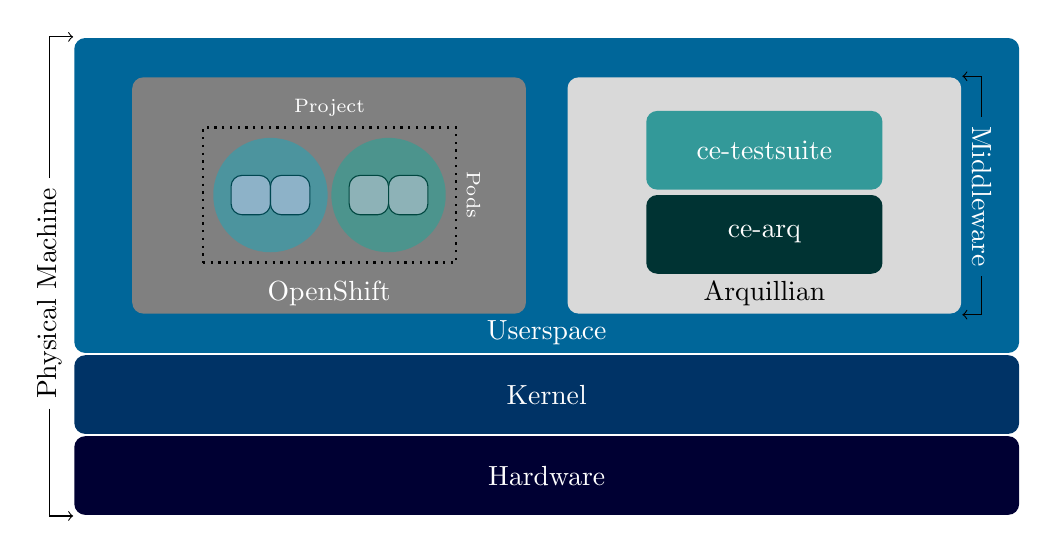
\begin{tikzpicture}[node distance = 1cm and 0cm]

  \tikzstyle{mw} = [minimum width= 12 cm]
  \tikzstyle{mh} = [minimum height= 1.0 cm]
  \tikzstyle{box} = [rectangle, thick, rounded corners, text= white]
  \tikzstyle{layer} = [box, mw, mh]

  \tikzstyle{OS_LAYER} = [box, OS_COLOR, minimum width = 3 cm, minimum height = 1 cm]

  \node[USR_COLOR, layer, minimum height = 4cm, label={[label distance=-0.55cm]270:\color{white}Userspace}] (USR) {};
  \node[KRN_COLOR, layer, below = 0cm of USR] (KRN) {Kernel};
  \node[HW_COLOR,  layer, below = 0cm of KRN] (HW) {Hardware};

  \tikzstyle{mw}  = [minimum width= 5 cm]
  \tikzstyle{mh}  = [minimum height= 3 cm]
  \xdef\dis{0.25}

  \node[OS_COLOR, layer,  mh, mw,  label={[label distance=-0.55cm]270:\color{white}OpenShift},
  left= \dis cm of USR.center] (OS) {};
  \node[ARQ_COLOR, layer, mh, mw,  label={[label distance=-0.55cm]270:\color{black}Arquillian},
  right= \dis cm of USR.center] (ARQ) {};

  \tikzstyle{mw} = [minimum width= 3 cm]
  \tikzstyle{mh} = [minimum height= 1 cm]

  \node[CE_ARQ_COLOR, layer,  mh, mw, below= -0.02cm of ARQ.center] (CE_ARQ) {ce-arq};
  \node[CET_COLOR, layer,  mh, mw, above= 0.06cm of ARQ.center] (CET) {ce-testsuite};

  \node[fit=(USR)(KRN)(HW)] (HOST) {};
  \node[rotate=90, above left = 1.25cm and -0.1cm of HOST.west ] (HM) {Physical Machine};
  \path[->, thin, to path={|- (\tikztotarget)}]
    (HM.west) edge (HW.south west)
    (HM.east) edge (USR.north west);

  \node[rotate=-90, above right = 1cm and 0.0cm of ARQ.east] (MW) {\color{white} Middleware};
  \path[->, thin, to path={|- (\tikztotarget)}]
    (MW.west) edge (ARQ.north east)
    (MW.east) edge (ARQ.south east);

  \project{PRJ0}{0.5}{4}{2}{above left = -0.5cm and 1.5cm of OS.center}
  \node[text= white,above= 0cm and 0cm of PRJ0.north, anchor=south] (PRJ_LABEL) {\scriptsize Project};
  \node[text=white, rotate=-90, right= 0cm and 0cm of PRJ0.east, anchor=south] (POD_LABEL) {\scriptsize Pods};

\end{tikzpicture}
\caption{Diagram of Platform Architecture} 
\end{figure}

The basis of this article relies upon the foundation of others
\begin{enumerate}[(1)]
 \item \href{https://kyguy.github.io/src/containers/containers.html}{Containers}
 \item \href{https://kyguy.github.io/src/openshift/openshift.html}{OpenShift}
\end{enumerate}
Read these first for a more in depth understanding \


--------------------------------------------------------------------------------------------------------------------- \\
 WIP \\
--------------------------------------------------------------------------------------------------------------------- \\

%================================================
% CONTAINER TESTING
%================================================
%\subsection{Container Testing}
%Testing Java code within containers can get pretty difficult, Arquillian is a custom testrunner 


%================================================
% CONTAINER TECHNOLOGY
%================================================
%\section{Middleware(WIP)}

%\noindent Currently, the Cloud Enablement team is Mobyizing several Red Hat middleware products:
%\begin{itemize}
%\item AMQ(Advanced Message Queuing)
%\item EAP(Enterprise Application Platform)
%\item JDG(JBoss Data Grid)
%\item Kieserver(Realtime Decision Server)
%\item Spark(Cluster Computing Framework)
%\item SSO(Single Sign-on)
%\item Tomcat(JBoss Webserver)
%\end{itemize} 
%\noindent 
%

\iffalse
I don't want this to happen
\begin{figure}
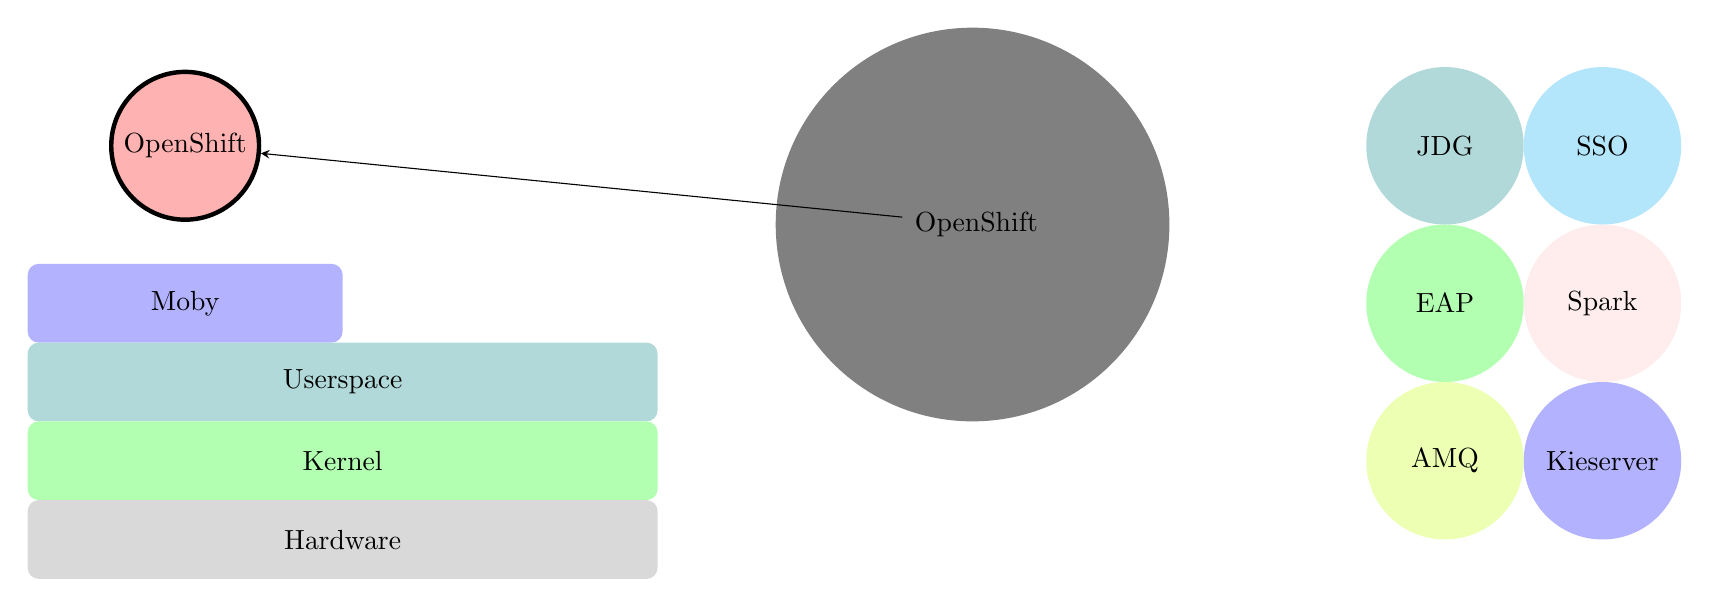
\begin{tikzpicture}[%
    >=stealth,
    node distance=0.05cm,
    on grid,
    auto
  ]
       %Stack
      \tikzstyle{core_stack}=[thick, rounded corners, minimum width=8cm,minimum height=1cm, rectangle]
      \tikzstyle{user_stack}=[ultra thick, rounded corners, minimum width=4cm,minimum height=1cm, rectangle]   
      \draw (-10, 2) node[user_stack, fill=red!30!white, state] (A) {OpenShift}; 
      %\draw (-10, 1) node[user_stack, fill=violet!30!white] {Kubernetes};
      \draw (-10, 0) node[user_stack, fill=blue!30!white] {Moby}; 
      \draw (-8, -1) node[core_stack,  fill=teal!30!white] {Userspace}; 
      \draw (-8, -2) node[core_stack,  fill=green!30!white] {Kernel};
      \draw (-8,-3) node[core_stack,  fill=gray!30!white] {Hardware};  
      
      %OpenShift Bubble
      \fill[black!50!white] (0,1) circle (2.5);
      
    
      %Red Hat Middleware Products
      \fill[lime!30!white] (6,-2) circle (1); %AMQ
      \fill[green!30!white](6,0) circle (1); %EAP
      \fill[teal!30!white] (6,2) circle (1); %JDG
      \fill[blue!30!white] (8,-2) circle (1); %Kieserver
      \fill[pink!30!white] (8,0) circle (1); %Spark
      \fill[cyan!30!white] (8,2) circle (1); %SSO
        %\fill[violet!30!white]  (360:2.5) circle (1); %Tomcat
      \node at (6,-2)    {AMQ};
      \node at (6,0)   {EAP};
      \node at (6,2)   {JDG};
      \node at (8,-2)   {Kieserver};
      \node at (8,0)   {Spark};
      \node at (8,2)   {SSO};
     
      %\node at (360:2.5)    {Tomcat};
      \node (B) [circle, right of=A] at (0,1) {OpenShift}; 
      \%path[->] (B) edge (A);
      \draw [->] (B) edge (A);
    \end{tikzpicture}
\end{figure}
 \fi
%%%%%%%%%%%%%%%%%%%%%%%%%%%%%%%%%%%%%%%%%%%%%%%%%
%%%%%%%%%%%%%%%%%%%%%%%%%%%%%%%%%%%%%%%%%%%%%%%%%

\iffalse
\section{Application Templates}
The application-templates can be found here \url{https://github.com/jboss-openshift/application-templates}

\begin{figure}
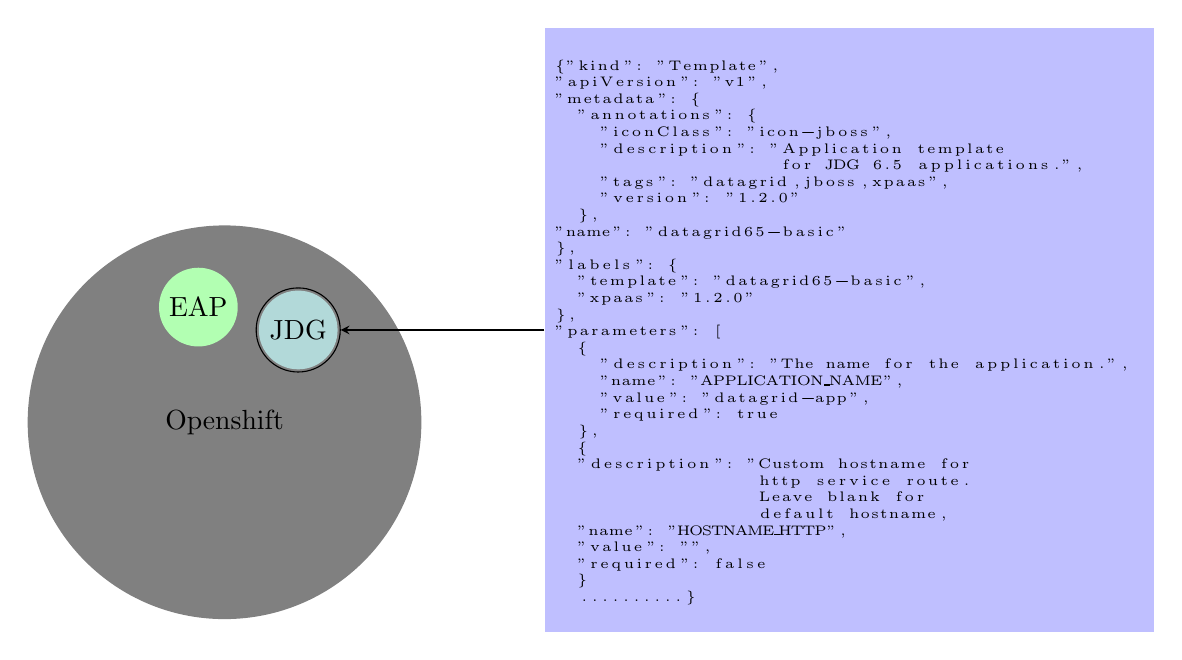
\begin{tikzpicture}[%
    >=stealth,
    node distance=7cm,
    on grid,
    auto
  ]
  \begin{scope}[blend group = soft light]
        %OpenShift Bubble
        \fill[black!50!white]   (0,0) circle (2.5);
  \end{scope}
  \begin{scope}[blend group = soft light]
    \fill[teal!30!white](51.4:1.5) circle (0.5); %JDG
    \fill[green!30!white](102.8:1.5) circle (0.5); %EAP
  \end{scope}
    \node[state] (A) at (51.4:1.5)  {JDG};
    \node at (102.8:1.5) {EAP};
    \node at (0,0)       {Openshift};
    \node (B) [right of=A,fill=blue!25,text width=7.5cm, font=\tiny]{ \begin{lstlisting}
{"kind": "Template",
"apiVersion": "v1",
"metadata": {
  "annotations": {
    "iconClass": "icon-jboss",
    "description": "Application template 
                    for JDG 6.5 applications.",
    "tags": "datagrid,jboss,xpaas",
    "version": "1.2.0"
  },
"name": "datagrid65-basic"
},
"labels": {
  "template": "datagrid65-basic",
  "xpaas": "1.2.0"
},
"parameters": [
  {
    "description": "The name for the application.",
    "name": "APPLICATION_NAME",
    "value": "datagrid-app",
    "required": true
  },
  {
  "description": "Custom hostname for 
                  http service route. 
                  Leave blank for 
                  default hostname,
  "name": "HOSTNAME_HTTP",
  "value": "",
  "required": false
  }
  ..........}
\end{lstlisting}
    };;
    \path[->] (B) edge (A);
  \end{tikzpicture}
\end{figure}
%%%%%%%%%%%%%%%%%%%%%%%%%%%%%%%%%%%%%%%%%%%%%%%%%

\section{Arquillian Components}
  
\begin{lstlisting}
@Test <---- Runs on client
public void testRestService() throws Exception {
  String host = System.getenv("DATAGRID_APP_SERVICE_HOST");
  int port = Integer.parseInt(System.getenv("DATAGRID_APP_SERVICE_PORT"));
  RESTCache<String, Object> cache = new RESTCache<>("default", new URL("http://" + host + ":" + port), "rest");
  cache.put("foo1", "bar1");
  assertEquals("bar1", cache.get("foo1"));
}
\end{lstlisting}


\begin{lstlisting}
|@Test|   
|@RunAsClient|
|@InSequence(1)|
public void testCarMartApp() throws Exception {
  Car car = new Car("test", 0.0, CarType.SEDAN, "test", "test", Country.USA);
  client = HttpClientBuilder.untrustedConnectionClient();
  addCar(car);
	assertCarsAreSame(car, getCar(car));
}
\end{lstlisting}

\noindent Before we dive into the details of the testsuite, we must first understand the Arquillian components. When maven builds an application, it spawns two JVMs; one for the testrunner and one for the tests. Take the following example for example

\begin{lstlisting}[style=Java]
|@Test|    <-------------- Local Test
|@RunAsClient|
|@InSequence(1)|
public void testCarMartApp() throws Exception {
  Car car = new Car("test", 0.0, CarType.SEDAN, "test", "test", Country.USA);
  client = HttpClientBuilder.untrustedConnectionClient();
  addCar(car);
	assertCarsAreSame(car, getCar(car));
}
\end{lstlisting}


\begin{lstlisting}
|@RunWith|(Arquillian.class)
|@Template|(url="https://raw.githubusercontent.com/jboss-openshift/application-templates/master/datagrid/datagrid65-basic.json")
|@RoleBinding|(roleRefName = "view", userName = "system:serviceaccount:\${kubernetes.namespace}:jdg-service-account")
|@OpenShiftResources|({
  |@OpenShiftResource|("https://raw.githubusercontent.com/\${template.repository:jboss-openshift}/application-templates/\${template.branch:master}/secrets/datagrid-app-secret.json")
})
public class JdgBasicTest extends JdgTestBase {
  |@Deployment|
  public static WebArchive getDeployment() {
    return getDeploymentInternal();
  }
}
\end{lstlisting}

  %\begin{scope}[blend group = soft light] 
        %\fill[lime!30!white] (51.4:2.5) circle (1); %AMQ
        %\fill[green!30!white] (102.8:2.5) circle (1); %EAP
        %\fill[teal!30!white]  (154.2:2.5) circle (1); %JDG
        %\fill[blue!30!white]  (205.7:2.5) circle (1); %Kieserver
        %\fill[pink!30!white]  (257.1:2.5) circle (1); %Spark
        %\fill[cyan!30!white]  (308.5:2.5) circle (1); %SSO
        %\fill[violet!30!white]  (360:2.5) circle (1); %Tomcat
      %\end{scope}
      %\node at (51.4:2.5)    {AMQ};
      %\node at (102.8:2.5)   {EAP};
      %\node at (154.2:2.5)   {JDG};
      %\node at (205.7:2.5)   {Kieserver};
      %\node at (257.1:2.5)   {Spark};
      %\node at (308.5:2.5)   {SSO};
      %\node at (360:2.5)    {Tomcat};
\fi
\end{document}
